\documentclass[]{article}

% Imported Packages
%------------------------------------------------------------------------------
\usepackage{amssymb}
\usepackage{amstext}
\usepackage{amsthm}
\usepackage{amsmath}
\usepackage{enumerate}
\usepackage{fancyhdr}
\usepackage[margin=1in]{geometry}
\usepackage{graphicx}
\usepackage{float}
%\usepackage{extarrows}
%\usepackage{setspace}
%\usepackage{xcolor}
\usepackage{color}
%------------------------------------------------------------------------------

% Header and Footer
%------------------------------------------------------------------------------
\pagestyle{plain}  
\renewcommand\headrulewidth{0.4pt}                                      
\renewcommand\footrulewidth{0.4pt}                                    
%------------------------------------------------------------------------------

% Title Details
%------------------------------------------------------------------------------
\title{Deliverable \#1 Template : Software Requirement Specification (SRS)}
\author{SE 3A04: Software Design II -- Large System Design}
\date{}
                            

%------------------------------------------------------------------------------

% Document
%------------------------------------------------------------------------------
\begin{document}
\setlength\parindent{0pt} 
\setlength{\parskip}{\baselineskip}

\maketitle	
\noindent{\bf Tutorial Number:} T0x\\
{\bf Group Number:} G07 \\
{\bf Group Members:} 
\begin{itemize}
	\item Farid Bastoros 
	\item Neha Bhatla
	\item 
	\item
	\item  
\end{itemize}

\section*{IMPORTANT NOTES}
\begin{itemize}
	\item Be sure to include all sections of the template in your document regardless whether you have something to write for each or not
	\begin{itemize}
		\item If you do not have anything to write in a section, indicate this by the \emph{N/A}, \emph{void}, \emph{none}, etc.
	\end{itemize}
	\item Uniquely number each of your requirements for easy identification and cross-referencing
	\item Highlight terms that are defined in Section~1.3 (\textbf{Definitions, Acronyms, and Abbreviations}) with \textbf{bold}, \emph{italic} or \underline{underline}
	\item For Deliverable 1, please highlight, in some fashion, all (you may have more than one) creative and innovative features. Your creative and innovative features will generally be described in Section~2.2 (\textbf{Product Functions}), but it will depend on the type of creative or innovative features you are including.
\end{itemize}

\newpage
\section{Introduction}
\label{sec:introduction}
% Begin Section

\begin{itemize}
	\item Provide an overview of the document/SRS.
\end{itemize}


\subsection{Purpose}
\label{sub:purpose}
% Begin SubSection
\begin{itemize}
	\item Specify the purpose of the SRS.
	\item Specify the intended audience for the SRS.
\end{itemize}
% End SubSection

\subsection{Scope}
\label{sub:scope}
% Begin SubSection
\begin{itemize}
	\item Identify the software product(s) to be produced, and name each (e.g., Host DBMS, Report Generator, etc.)
	\item Explain what the software product(s) will do (and, if necessary, also state what they will not do).
	\item Describe the application of the software being specified, including relevant benefits, objectives, and goals.
%	\item Be consistent with similar statements in higher-level specifications (e.g., the system requirements specification), if they exist
\end{itemize}

\noindent
Mushroom.id, the mushroom identification application will allow users to identify mushrooms based on data collected in the field while foraging. The application is expected to use three
independent sources of identification called "experts". The experts are not intended to be real individuals, but rather software components that will provide identification based on user provided data. 

\vspace{0.5cm}
\noindent
The three experts are expected to be:

\begin{itemize}
	\item Macro Photo Expert: This expert will use a photo of the mushroom taken using a camera to identify the mushroom. THe user will be required to take a photo of the mushroom and upload it to be the application. The expert based on a CNN (Convolutional Neural Network) will identify the mushroom along with a probability.
	\item Micro Photo Expert: This expert will use a photo of the mushroom taken using a microscope to identify the mushroom. The user will be required to take a photo of the mushroom under a microscope and upload it to the application. The expert based on a CNN (Convolutional Neural Network) will identify the mushroom along with a probability.
	\item Text Description Expert: This expert will use textual descriptions of the mushroom, the location of the mushroom and other relevant information to identify the mushroom. The user will be required to input the textual information into the application. The expert based on a NLP (Natural Language Processing) model will identify the mushroom along with a probability.
\end{itemize}

Mushroom.id is not expected to provide any guarantees regarding the classification of the mushrooms, only a confidence percentage with a classification ranging from 0-100\%
Each expert module is expected to output a confidence probability ranging from 0.0 to 1.0 and a forum component will use each output and confidence probability to make the final decision.

If the user chooses to accept the mushroom identification outputted by the application, the application will also provide the user with a list of similar mushrooms and recipes that can be prepared using the identified mushroom.

To use the application the user is required to create an account so that the application can create a profile for the user to store their previous identifications and preferences. The user will also be able to access the application without creating an account, but the application will not store any of the user's data.
% End SubSection

\subsection{Definitions, Acronyms, and Abbreviations}
\label{sub:definitions_acronyms_and_abbreviations}
% Begin SubSection
\begin{itemize}
	\item Provide the definitions of all terms, acronyms, and abbreviations required to properly interpret the SRS.
	\item This should be in alphabetical order.
\end{itemize}
% End SubSection

\subsection{References}
\label{sub:references}
% Begin SubSection
\begin{itemize}
	\item Provide a complete list of all documents referenced elsewhere in the SRS.
	\item Identify each document by title, report number (if applicable), date, and publishing organization.
	\item Specify the sources from which the references can be obtained.
	\item Order this list in some sensible manner (alphabetical by author, or something else that makes more sense).
\end{itemize}
% End SubSection

\subsection{Overview}
\label{sub:overview}
% Begin SubSection

Section 2 will be discussing the overall product description and describe the general factors that affect the product. This will include product perspective and functions, user characteristics, assumptions and dependencies, and apportioning of requirements. Section 3 includes a Use Case Diagram for the scenario of identifying a mushroom in the wild. Section 4 highlights the function requirements and specifies all the uses cases by their Business Events. Section 5 will then move on to Non-Functional requirements, discussing look and feel, usability and humanity, performance, security, and cultural and political requirements. Finally, section A contains a division of labour.

% End SubSection

% End Section

\section{Overall Product Description}
\label{sec:overall_description}
% Begin Section

\begin{itemize}
	\item This section should describe the general factors that affect the product and its requirements. 
	\item It does not state specific requirements.
	\item It provides a \emph{background} for those requirements and makes them easier to understand.
\end{itemize}


\subsection{Product Perspective}
\label{sub:product_perspective}
% Begin SubSection
[Name] is a mobile mushroom identification app that allows users to submit a text description, macro photo, or micro photo of a mushroom and get detailed information on it. It will function similarly to Google Lens which lets users identify objects with their camera, but it will be specifically tailored to fungi allowing for more accuracy. The product will use state of the art machine learning-based services to determine the species. Location data will be used to narrow down the results, allowing for more accuracy. Users will have a profile where they can save their mushrooms, similar to a Pokedex.\\

The system will interact with Plant.id's identification api and [SYSTEM FOR ANALYZING TEXT DATA] in order to determine the specific fungi and if it is edible. It will be clarified to the user that they are only to consume the mushrooms at their own risk. If the mushroom is determined to be edible, the product will recommend recipes the user can cook using said mushroom. \\

\begin{figure}[h!]
    \centering
    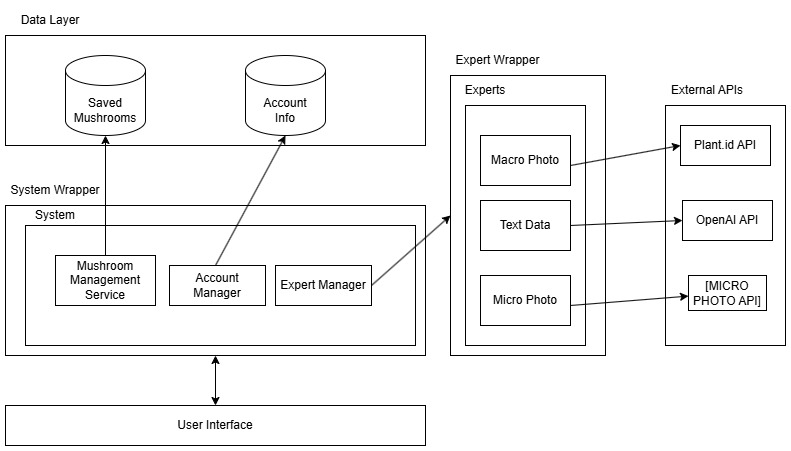
\includegraphics[width=0.9\textwidth]{BlockDiagram.jpg}
    \caption{System Diagram.}
    \label{fig:example}
\end{figure}
% End SubSection

\subsection{Product Functions}
\label{sub:product_functions}
% Begin SubSection
\begin{itemize}
	\item Provide a \emph{summary} of the major functions that the software will perform.
	\begin{itemize}
		\item \textbf{Example}: An SRS for an accounting program may use this part to address customer account maintenance, customer statement, and invoice preparation without mentioning the vast amount of detail that each of those functions requires.
	\end{itemize}
	\item Functions should be organized in a way that makes the list of functions understandable to the customer or to anyone else reading the document for the first time 
	\item Present the functions in a list format - each item should be one function, with a brief description of it
	\item Textual or graphical methods can be used to show the different functions and their relationships
	\begin{itemize}
		\item Such a diagram is not intended to show a design of a product, but simply shows the logical relationships among variables
	\end{itemize} 
\end{itemize}
% End SubSection

\begin{table}[H]
	\centering
	
	\label{tab:product_functions}
	\begin{tabular}{|c|p{10cm}|}
		\hline
		\textbf{Modules} & \textbf{Functions} \\
		\hline
		\hline
		\textbf{Decision Forum} & \begin{itemize}
			\item Mushroom Identification: The decision forum shall poll experts based on inputs provided to attempt to identify a mushroom.
			\item User Input: The decision forum shall accept three user inputs - a macro photo, a micro photo, and a text description and validate the inputs.
			\item Voting: The decision forum shall poll the experts and output a final decision based on the expert's outputs and confidence probabilities.
		\end{itemize} \\
		\hline
		\textbf{Account Manager} & \begin{itemize}
			\item Account creation: The account manager shall allow users to register and create an account.
			\item Account deletion: The account manager shall allow users to delete their account.
			\item Account modification: The account manager shall allow users to modify their account.
			\item Account login/logout: The account manager shall allow users to login and logout of their account.
		\end{itemize} \\
		\hline
		\textbf{Recipe Recommender} & \begin{itemize}
			\item Recipe Identification: The recipe recommender shall recommend a list of recipes based on the identified mushroom.
			\item Recipe Filtering: The recipe recommender shall allow users to filter the list of recipes based on dietary restrictions.
			\item Recipe Favoriting: The recipe recommender shall allow users to favorite recipes.
		\end{itemize} \\
		\hline
	\end{tabular}
	\caption{Product Functions}
\end{table}

\subsection{User Characteristics}
\label{sub:user_characteristics}
% Begin SubSection
General characteristics of the intended users of the product:
\begin{enumerate}
	\item Education Level: Basic Literacy required
	\begin{itemize}
		\item Users with the ability to read, write, and comprehend simple instructions should face no problems using the app.
	\end{itemize}
	\item Experience: No prior experience required
	\begin{itemize}
		\item First-time users should be able to navigate without difficulty, as the app is assumed to be user-friendly.
	\end{itemize}
	\item Technical Expertise: Familiarity with touchscreen devices
	\begin{itemize}
		\item Users with basic knowledge of touchscreen interactions, such as swiping, tapping, and typing, should have no issues using the app.
	\end{itemize}
\end{enumerate}
% End SubSection

\subsection{Constraints}
\label{sub:constraints}
% Begin SubSection
\begin{itemize}
	\item Provide a general description of any constraints that will limit the developer's options
\end{itemize}
% End SubSection

\subsection{Assumptions and Dependencies}
\label{sub:assumptions_and_dependencies}
% Begin SubSection
Assumptions made while interpreting what the software being developed aims to achieve.
\begin{enumerate}
	\item The function of identifying a mushroom is different from discovering the different types of mushrooms.
	\item \textbf{\textcolor{red}{Innovative feature 1:}} The user can collect mushrooms. When they identify one, it's saved to their account as a collected mushroom.
	\item \textbf{\textcolor{red}{Innovative feature 2:}} After the user has found an edible mushroom, they can find recipes for it.
	\item Assume "Identify Mushroom using photo" implies displaying the camera app to take a picture.
	\item The app will only be used in Canada.
\end{enumerate}

Other assumptions that, if it fails to hold, could require a change to the requirements:
\begin{enumerate}
	\item The product shall have uninterrupted access to an internet connection.
    \item Assume that users have granted all necessary permissions for the app to function properly.
    \item Assume that third-party libraries and dependencies remain compatible with future updates.
    \item Assume that APIs remain compatible with future updates.
\end{enumerate}
% End SubSection

\subsection{Apportioning of Requirements}
\label{sub:apportioning_of_requirements}
% Begin SubSection
\begin{itemize}
	\item \textbf{Varying Language Options:} The initial version of the app only supports English; however, in the future, additional language options will be implemented to create a more inclusive environment for a broader user base.
	\item \textbf{Offline Usage:} The initial release of the application will require an internet connection to identify mushrooms. Future versions may include an offline identification feature, allowing users to access identification tools without being connected to an internet network.
	\item \textbf{VR/AR for Mushroom Identification:} In the initial release, the app will rely on macro and micro photos for identification, with users being presented with a new screen of information regarding the identified mushroom. A future update may include augmented reality (AR) functionality that overlays information about mushrooms directly onto the camera’s view in real time.
	\item \textbf{Competitive Gameplay:} While the initial version focuses on individual mushroom identification, future updates may include competitive gaming features to create a more engaging experience for users. This could be implemented with a leaderboard ranking users based on the number of mushrooms identified or rare mushroom discoveries.
\end{itemize}
% End SubSection

% End Section
\section{Use Case Diagram}
\label{sec:use_case_diagram}
% Begin Section
\begin{itemize}
	\item Provide the use case diagram for the system being developed.
	\item You do not need to provide the textual description of any of the use cases here (these will be specified under "Highlights of Functional Requirements").
%	\item Provide \emph{one} use case diagram for the most important Business Event.
%	\item The text of all use cases will be specified under "Highlights of Functional Requirements"
\end{itemize}
%In this section, select the most important Business Event that your system responds to and give its use case diagram.  Only one use case diagram is needed.  Give a brief textual description of the use case without repeating what is in the scenarios of the corresponding Business Event.

%
%
%
%This section should provide a use case diagram for your application. 
%\begin{enumerate}[a)]
%	\item Each use case appearing in the diagram should be accompanied by a text description. 
%\end{enumerate}
%% End Section

\section{Highlights of Functional Requirements}
\label{sec:functional_requirements}
% Begin Section
\begin{itemize}
	\item Specify all use cases (or other scenarios triggered by other events), organized by Business Event. 
	\item For each Business Event, show the scenario from every Viewpoint. You should have the same set of Viewpoints across all Business Events. If a Viewpoint doesn't participate, write N/A so we know you considered it still. You can choose how to present this - keep in mind it should be easy to follow. 
	\item At the end, combine them all into a Global Scenario.
	%\item Specify the "use cases" (or other triggering events) organized by Business Event. (The Global Scenario is what you might think of as a use case). Be sure to consider Business Events that aren't just triggered by users with goals (e.g. something happens in the environment that your system needs to respond to)
	\item Your focus should be on what the system needs to do, not how to do it. Specify it in enough detail that it clearly specifies what needs to be accomplished, but not so detailed that you start programming or making design decisions.
	\item Keep the length of each use case (Global Scenario) manageable. If it's getting too long, split into sub-cases.
	\item You are \emph{not} specifying a complete and consistent set of functional requirements here. (i.e. you are providing them in the form of use cases/global scenarios, not a refined list). For the purpose of this project, you do not need to reduce them to a list; the global scenarios format is all you need.
	\item Red text below is just to highlight where you need to insert a scenario - don't actually write it all in red.
\end{itemize}

\noindent {\bf Main Business Events:} List out all the main business events you are presenting. If you sub-divided into smaller ones, you don't need to include the smaller ones in this list.\\

\begin{itemize}
	\item BE1: Identify a mushroom.
 	\item BE2. Save Mushroom to Profile.
\end{itemize}

\noindent {\bf Viewpoints:} List out all the viewpoints you will be considering.\\

\begin{itemize}
	\item VP1: User
	\item VP2: External Providers
	\item VP3: Marketing
	\item VP4: Mycologist (Fungi expert)
	\item VP5: Culinary Expert
\end{itemize}

\noindent {\bf Interpretation:} Specify any liberties you took in interpreting business events, if necessary.\\

\begin{enumerate}[{\bf BE1.}]
	\item Identify a mushroom. \\
	\\
	\textbf{Pre-condition}: User has the app opened and has completed initial app setup. 
		\begin{enumerate}[{\bf VP1.}]
			\item User \#1 \\
				\textbf{Main Scenario:}
				\begin{enumerate}[1.]
					\item User taps the button to open the mushroom identification page.
					\item The user presses the button to upload images.
					\item The system displays all images stored in the phone gallery.
					\item The user selects and confirms the desired macro and micro image of the mushroom.
					\item The system confirms if the pictures are valid and usable.
					\item The system uploads the image to the macro and micro image identifier expert and displays a checkmark to the user.
					\item The user selects the option to fill out the form for the textual identification expert. 
					\item The system displays the form to the user.
					\item The user fills out the form with a description of the mushroom and GPS location.
					\item The system verifies the form and uploads it to the textual identification expert.
					\item User requests the identification process to begin.
					\item Once a decision has been reached, the system displays the resulting identification and confidence probability.
				\end{enumerate}
			\item External Provider\\
				\begin{enumerate}[1.]
					\item The external system receives an image upload request.
					\item System begins transferring images for the image based experts.
					\item System sends back upload complete and successful message to client.
					\item System recieves a completed form to store.
					\item System sends back success message to client.
					\item System receives a request to start identification process.
					\item System validates inputs provided and starts the identification process.
					\item Once the decision forum reaches a final decision, the system sends the results to the client.
				\end{enumerate}
			\item Marketing\\
				\textcolor{red}{N/A}
			\item Mycologist\\
				\begin{enumerate}[1.]
					\item Mycologist wants to ensure an overall decision system accuracy rate.
				\end{enumerate}
			\item Culinary Expert\\
				\textcolor{red}{N/A}
		\end{enumerate}
		
		\vspace{0.2cm}
		\textbf{Post condition: } User has received mushroom identification results with a confidence level.\\
		\vspace{0.1cm}\\
		{\bf Global Scenario:}\\
		\begin{enumerate}[1.]
			\item User taps the button to open the mushroom identification page.
			\item The user presses the button to upload images.
			\item The system displays all images stored in the phone gallery.
			\item The user selects and confirms the desired macro and micro image of the mushroom.
			\item The system confirms if the pictures are valid and usable.
			\item The system uploads the image to the macro and micro image identifier expert.
			\item External provider system receives an image upload request.
			\item External provider system begins transferring images for the image based experts.
			\item External provider system sends back upload complete and successful message to client.
			\item The system displays a checkmark to the user confirming success.
			\item The user selects the option to fill out the form for the textual identification expert. 
			\item The system displays the form to the user.
			\item The user fills out the form with a description of the mushroom and GPS location.
			\item The system verifies the form and uploads it to the textual identification expert.
			\item External provider system recieves a completed form to store.
			\item External provider systems sends a success message to client.
			\item User requests the identification process to begin.
			\item External provider system receives a request to start identification process.
			\item External provider system validates inputs provided and starts the identification process.
			\item Identification results are further validated based on heuristics provided by Mycologist.
			\item Once the decision forum reaches a final decision, the result is sent to the client.
		\end{enumerate}
	\item Save Mushroom to Profile \#2\\
	    \textbf{Pre-condition:} The user is logged in and viewing a mushroom identification result.\\[1mm]
	    
	    \textbf{VP1. User \#1}\\
	    \textbf{Main Success Scenario:}
	    \begin{enumerate}
	        \item[1.] System displays the mushroom identification result with a ``Save to Profile'' option.
	        \item[2.] User selects the ``Save to Profile'' option.
	        \item[3.] Mushroom data is sent to the Database for storage.
	        \item[4.] System updates the user's profile with the mushroom information and displays a confirmation message.
	    \end{enumerate}
	    \textbf{Secondary Scenario:}
	    {\color{red}
	    \begin{enumerate}
	        \item[2i.] The system fails to update the user profile with the mushroom information.
	        \begin{enumerate}
	            \item[2i.1] The system attempts to retry the update operation.
	            \item[2i.2] If the retry fails, the system displays an error message indicating that the save operation was unsuccessful. 
	        \end{enumerate}
	        \item[3i.] Database fails to upload the Mushroom Information.
	        \begin{enumerate}
	            \item[3i.1] The system attempts to retry the database upload.
	            \item[3i.2] If unsuccessful, the system displays an error message indicating that the database upload failed.
	        \end{enumerate}
	    \end{enumerate}
	    }
	    \textbf{VP2. External Services (Database/API) \#2}
	    {\color{red}
	        \begin{enumerate}
	        \item[3i.] Database error message is received, logged, and troubleshooted.
	    \end{enumerate}
	    }
	    \textbf{VP3. Customer Support \#3}
	        {\color{red}
	        \begin{enumerate}
	        \item[2i.] System should prompt an error page with suggestions to retry the operation or provide a link to contact customer support.\\
	    \end{enumerate}
	    }
	    \textbf{VP4. Marketing \#4}\\
	    NA\\[1mm]
	    
	    \textbf{VP5. Mushroom Expert \#5}\\
	    NA\\[1mm]
	    
	    \textbf{Global Scenario:}\\
	    \textbf{Pre-condition:} The user is logged in and a mushroom identification result is available.\\[1mm]
	    \textbf{Main Success Scenario:}
	    \begin{enumerate}
	        \item[1.] System displays the mushroom identification result with a ``Save to Profile'' option.
	        \item[2.] User selects the ``Save to Profile'' option.
	        \item[3.] Mushroom data is sent to the Database for storage.
	        \item[4.] System updates the user's profile with the mushroom information and displays a confirmation message.
	    \end{enumerate}
	    \textbf{Secondary Scenario:}
	    {\color{red}
	    \begin{enumerate}
	        \item[2i. ] The system fails to update the user profile with the mushroom information.
	        \begin{enumerate}
	            \item[2i.1] The system attempts to retry the update operation.
	            \item[2i.2] If the retry fails, the system displays an error message indicating that the save operation was unsuccessful. 
	        \end{enumerate}
	        \item[3i.] Database fails to upload the Mushroom Information.
	        \begin{enumerate}
	            \item[3i.1] The system attempts to retry the database upload.
	            \item[3i.2] If unsuccessful, the system displays an error message indicating that the database upload failed.
	        \end{enumerate}
	    \end{enumerate}
	    }

		\item Recipe Recommendation \\
		\\
		\textbf{Pre-condition}: User has identified a mushroom and it is classified as safe for consumption. The user has an active account.
		\begin{enumerate}[{\bf VP1.}]
			\item VP1: User \#1 \\
		\textbf{Main Success Scenario} 
			\begin{enumerate}
				\item[1.] User navigates to the Recipe Recommendation page.
				\item[2.] System checks if the identified mushroom is edible.
				\item[3.] System fetches curated recipes that involve the identified mushroom.
				\item[4.] System displays a list of recipe options with preparation details and ingredient lists.
				\item[5.] User selects a recipe to view cooking steps in detail.
				\item[6.] System provides step-by-step cooking instructions along with safety tips.
				\item[7.] User has the option to save the recipe for later or share it with others.
			\end{enumerate}
			
			\textbf{Secondary Scenario}
			\begin{enumerate}
				\item[3i.] No recipes found for the mushroom.
				\begin{enumerate}
					\item[3i.1] System notifies the user that no recipes are available.
					\item[3i.2] System suggests searching for other edible mushrooms.
				\end{enumerate}
				\item[4i.] User selects a recipe, but the link is broken.
				\begin{enumerate}
					\item[4i.1] System displays an error message and offers alternative recipes.
				\end{enumerate}
				\item[5i.] Mycologist reports an error in mushroom classification.
				\begin{enumerate}
					\item[5i.1] System removes the recipe and warns the user.
				\end{enumerate}
			\end{enumerate}
			
			\item VP2: External Provider \#2 \\
				\textbf{Main Success Scenario} 
			\begin{enumerate}
				\item[1.] External system provides API data for recipes.
				\item[2.] System fetches and updates recipe recommendations.
			\end{enumerate}
			 \textbf{Secondary Success Scenario}
			  \begin{enumerate}
				\item[1i.] External system API is unavailable.
					\begin{enumerate}
						 \item[1i.1] System notifies the user that recipe recommendations cannot be updated.
						 \item [1i.2] System suggests trying again later or browsing previously saved recipes.
					\end{enumerate}
					\item[2i.] External system returns incomplete or invalid data. previously saved recipes.
					\begin{enumerate}
						 \item[2i.1] System logs the error and excludes incomplete data from the recommendations.
						 \item[2i.2] System notifies the user of potential missing recipes and offers existing curated options.
					\end{enumerate}
			\end{enumerate}
			
			\item VP3: Marketing \#3 \\ 
				\textbf{Main Success Scenario} 
			\begin{enumerate}
				\item[1.] User has the option to share the recipe with others through social media.
			\end{enumerate}
				\textbf{Secondary Success Scenario}
				\begin{enumerate}
				\item[1i.] System fails to connect to the selected social media platform.
					\begin{enumerate}
						 \item[1i.1] System notifies the user of the issue and suggests trying again later.
					\end{enumerate}
				\end{enumerate}
				
			\item VP4: Mycologist \#4 \\
				\textbf{Main Success Scenario} 
			\begin{enumerate}
				\item[1.] Mycologist ensures that the system only recommends safe mushrooms.
					\item[2.] System updates recommendations based on the mycologist's approval.
			\end{enumerate}
				\textbf{Secondary Success Scenario}
				\begin{enumerate}
				\item[1i.1] Mycologist identifies a misclassified mushroom.
					\item[1i.2] System removes the related recipes and notifies users who saved or interacted with them.
				\end{enumerate}
			
			\item VP5: Culinary Expert \#5 \\
				\textbf{Main Success Scenario} 
			\begin{enumerate}
				\item[1.] Culinary expert curates and verifies the quality of recommended recipes.
			\end{enumerate}
				\textbf{Secondary Success Scenario} 
			\begin{enumerate}
				\item[1i.1] Culinary expert curates and verifies the quality of recommended recipes.
					\item[1i.2] System removes the flagged recipe and notifies the users who saved or interacted with it.
			\end{enumerate}                    
		\end{enumerate}
			
			\textbf{Post-condition}:  
			\begin{itemize}
				\item User has successfully found a recipe and received cooking steps.
			\end{itemize}
			
			\textbf{Global Scenario:} \\
				\textbf{Pre-condition}: User has identified a mushroom and it is classified as safe for consumption. The user has an active account.
			\begin{enumerate}
				\item[1.] User navigates to the Recipe Recommendation page.
				\item[2.] System verifies if the mushroom is safe to eat.
				\item[3.] System retrieves a list of appropriate recipes.
				\item[4.] User selects a recipe and follows the cooking instructions.
				\item[5.] System records user interactions for future recipe recommendation improvements.
			\end{enumerate}

	\item Sharing on Social Media \#4\\
	
	\textbf{Pre-Condition:}\\
	The user has successfully identified a mushroom using the application. The user has an account and has access to at least one social media platform.\\
	
	\begin{enumerate}[{\bf VP1.}]
		\item User \#1 \\
		
		\textbf{Main Success Scenario} \\
		1. The user selects the "Share on Social Media" option after identifying an object. \\
		2. The system displays a list of supported platforms (e.g., Facebook, Instagram). \\
		3. The user selects a preferred platform for sharing. \\
		4. The system requests authentication if the user is not already logged in. \\
		5. Upon successful authentication, the system submits the post to the selected platform. \\
		6. The system generates an auto-formatted post, including an image, object details, and a brief description. \\
		7. The user customizes the post by adding a caption, hashtags, or tagging friends. \\
		8. The user sumbit the post to be shared.\\
		9. The user receives confirmation that the post was successfully shared. \\
		
		\textbf{Secondary Scenario} \\
		4i. System fails to authenticate the user. \\ 
		4i.1 The authentication process fails due to incorrect credentials.\\
		4i.2 The system prompts the user to retry or reset their password. \\ 
		4i.3 If multiple failed attempts occur, the system suggests contacting support. \\

		5i. System fails to connect to the selected social media platform.\\
		5i.1 The API request is rejected due to platform downtime or permission errors. \\
		5i.2 The system informs the user and suggests alternative sharing options. \\
		5i.3 The system saves the post in a queue to retry later. \\
		
		7i. User enters invalid post content. \\
		7i.1 The system detects restricted words or prohibited content.\\
		7i.2 The system notifies the user and requests modifications.\\
		7i.3 The user edits the post and resubmits it.\\

		\item External Providers (Social Media Platforms and APIs) \#2 \\
		
		\textbf{Main Success Scenario} \\
		1. The system sends a post request to the selected social media platform’s API.\\
		2. The external provider validates the request for format and compliance.\\
		3. The platform processes and schedules the content for posting.\\
		4. The provider returns a success response confirming the post is published.\\
		5. The platform allows users to interact with the post through likes, comments, and shares.\\
		6. The system logs the response for future tracking and analytics.\\
		
		\textbf{Secondary Scenario} \\
		1i. System fails to connect to the selected social media platform.\\
		1i.1 The API request is rejected due to platform downtime or permission errors. \\
		1i.2 The system informs the user and suggests alternative sharing options. \\
		1i.3 The system saves the post in a queue to retry later. \\
		
		\item Marketing \#3 \\
		
		\textbf{Main Success Scenario} \\
		1. The marketing team tracks user engagement metrics on social media. \\
		2. The system collects data on shared posts, including reach, impressions, and interactions.\\
		3. The team analyzes the data to understand sharing trends and user demographics.\\
		4. Insights are used to optimize promotional strategies and improve app visibility.\\
		5. The marketing team develops targeted campaigns encouraging more social sharing.\\
		6. Influencers or key users with high engagement are identified for potential collaborations.\\

		\textbf{Secondary Scenario} \\
		2i. The system fails to track user engagement data accurately.\\
		2i.1 The system fails to collect data on shared posts, including reach, impressions, and interactions.\\
		2i.2 The analysis process is impacted due to incomplete or inaccurate data.\\
		2i.3 Insights derived from the engagement metrics are unreliable, leading to ineffective promotional strategies.\\
		2i.4 The marketing team identifies the issue and implements corrective actions, such as refining data collection mechanisms or integrating third-party analytics tools.\\

		\item Fungi Expert \#4 \\
		
		\textbf{Main Success Scenario} \\
		1. A fungi expert discovers a shared post related to an identified mushroom.\\
		2. They verify the accuracy of the identification using the provided details.\\
		3. They engage by commenting with additional information.\\
		4. The expert shares related educational content to increase public knowledge.\\
		5. If necessary, they report misinformation to the app’s support team.\\
		
		\textbf{Secondary Scenario} \\
		3i. Fungi expert fails to engage with the post.\\
		3i.1 The expert’s comment fails to post due to restricted words or prohibited content.\\
		3i.2 The system flags the comment as potentially violating community guidelines.\\
		3i.3 The expert is prompted to edit and resubmit the comment.\\

		4i. The expert encounters difficulties sharing educational content.\\
		4i.1 The content-sharing feature malfunctions or experiences downtime.\\
		4i.2 The system informs the expert and suggests retrying later.\\
		4i.3 The expert is given the option to save the content as a draft.\\

		5i. The misinformation report submission fails.\\
		5i.1 The report submission does not go through due to a system error.\\
		5i.2 The expert is notified and given the option to retry.\\
		5i.3 The system saves the report and automatically resubmits it later.\\

		\item Cooking Expert \#5 \\
		
		\textbf{Main Success Scenario} \\
		1. A cooking expert finds a shared post about an edible mushroom. \\
		2. They verify the information to ensure it is correctly identified as safe.\\
		3. The expert engages by suggesting cooking methods or preservation techniques.\\
		4. They share additional culinary content, such as recipes or food pairings.\\
		5. If the mushroom has unique nutritional benefits, they highlight its value.\\
		6. The expert may reshare the post to food communities to expand reach.\\
		
		\textbf{Secondary Scenario} \\
		3i. Cooking expert fails to engage with the post.\\
		3i.1 The expert’s comment fails to post due to restricted words or prohibited content.\\
		3i.2 The system flags the comment as potentially violating community guidelines.\\
		3i.3 The expert is prompted to edit and resubmit the comment.\\

		4i. The expert encounters difficulties sharing educational content.\\
		4i.1 The content-sharing feature malfunctions or experiences downtime.\\
		4i.2 The system informs the expert and suggests retrying later.\\
		4i.3 The expert is given the option to save the content as a draft.\\

	\end{enumerate}
	{\bf Global Scenario:}\\

	\textbf{Pre-Condition:}\\
	The user has successfully identified a mushroom within the application. The user has an account and has access to at least one social media platform.\\
	
	\textbf{Main Success Scenario} \\
	1. The user selects the \textbf{Share on Social Media} option after identification.\\
	2. The system prompts the user to log in (if not already authenticated).\\
	3. The user enters their account credentials.\\
	4. The system authenticates the user.\\
	5. The system provides sharing options, including supported social media platforms.\\
	6. The user selects a preferred platform for sharing.\\
	7. The system generates an auto-formatted post containing an image, object details, and a description.\\
	8. The user customizes the post with a caption, hashtags, or tagged friends.\\
	9. The system sends the post request to the selected social media platform’s API.\\
	10. The external platform processes the request and publishes the post.\\
	11. The system confirms successful sharing and notifies the user.\\
	
	\textbf{Secondary Scenario}\\
	4i. System fails to authenticate the user.\\
	4i.1 The authentication process fails due to incorrect credentials.\\
	4i.2 The system prompts the user to retry or reset their password.\\
	4i.3 If multiple failed attempts occur, the system suggests contacting support.\\

	8i. User enters invalid post content.\\
	8i.1 The system detects restricted words or prohibited content.\\
	8i.2 The system notifies the user and requests modifications.\\
	8i.3 The user edits the post and resubmits it.\\

	9i. System fails to connect to the selected social media platform.\\
	9i.1 The API request is rejected due to platform downtime or permission errors.\\
	9i.2 The system informs the user and suggests alternative sharing options.\\
	9i.3 The system saves the post in a queue to retry later.\\
	
	\textbf{Post-Condition:}\\
	The user receives a confirmation message indicating that the post was published.


    \item Account Registration \\

\textbf{Pre-condition}: User does not have an existing account and the app is installed on their device.  

\begin{enumerate}[{\bf VP1.}]
    \item User \#1 \\
	\textbf{Main Success Scenario}
	\begin{enumerate}
		\item[1.] User navigates to the Sign-Up page.
		\item[2.] System prompts the user to enter required details:
		\begin{itemize}
			\item Full Name
			\item Email Address
			\item Password
			\item (Optional) Location for improved mushroom identification accuracy.
		\end{itemize}
		\item[3.] User enters details and presses “Create Account.”
		\item[4.] System verifies the input:
		\begin{itemize}
			\item Checks if the email is valid.
			\item Ensures the password meets security requirements.
			\item Confirms the email is not already in use.
		\end{itemize}
		\item[5.] System creates the account and sends a verification email.
		\item[6.] User verifies their email by clicking the confirmation link.
		\item[7.] System activates the account and redirects the user to the home page.
	\end{enumerate}

	\textbf{Secondary Scenario}
	\begin{enumerate}
		\item[3i.] User enters an invalid email format.
		\begin{enumerate}
			\item[3i.1] System prompts the user to enter a valid email.
		\end{enumerate}
		\item[3ii.] Password does not meet security requirements.
		\begin{enumerate}
			\item[3ii.1] System displays password guidelines.
		\end{enumerate}
		\item[4i.] Email is already registered.
		\begin{enumerate}
			\item[4i.1] System suggests the user logs in instead.
		\end{enumerate}
		\item[5i.] User does not receive verification email.
		\begin{enumerate}
			\item[5i.1] System allows resending the verification email.
		\end{enumerate}
		\item[6i.] User does not verify the email.
		\begin{enumerate}
			\item[6i.1] System reminds the user after 24 hours.
		\end{enumerate}
	\end{enumerate}

    \item External Provider \#2 \\
        \textbf{Main Success Scenario}
	\begin{enumerate}
		\item [1. ]External provider handles authentication services.
            \item [2. ] System grants the user access to the application features.
	\end{enumerate}
        \textbf{Secondary Scenario}
	\begin{enumerate}
		\item [1i. ]External provider fails to authenticate the user.
            \item [1i.1 ] System notifies the user of the issue and suggests retrying or resetting their password.
	\end{enumerate}      
        
 \item Marketing \#3 \\
	\textbf{N/A}

\item Customer Support \#4 \\
	\textbf{N/A}  

\item Customer Success \#5 \\
    \textbf{Main Success Scenario}
    \begin{enumerate}
		\item Displays customer satisfaction form.
    \end{enumerate}
    \textbf{Secondary Scenario}
   \begin{enumerate}
		\item[1i.] System fails to load the customer satisfaction form.
            \item[1i.1] System notifies the user of the issue and suggests retrying later.
            \item[1i.2] System logs the error for troubleshooting and provides an alternative feedback option (e.g., email support).
    \end{enumerate} 
	\textbf{Global Scenario:} \\
	\textbf{Post-condition}:  User successfully registers and verifies their account.

	\begin{enumerate}
		\item[1.] User navigates to Sign-Up.
		\item[2.] System prompts the user to enter details.
		\item[3.] User submits their information.
		\item[4.] System validates the input.
		\item[5.] System creates the account and sends a verification email.
		\item[6.] User verifies the email and logs in.
		\item[7.] System activates the account and grants access.
	\end{enumerate}


\end{enumerate}


%	Below, we organize by Business Event.
%	\begin{enumerate}[{BE}1.]
%		\item Business Event name
%		\begin{enumerate}[{VP1}.1]
%			\item Viewpoint name \newline
%			\noindent\fbox{%
%				\parbox{0.5\textwidth}{%
%					\begin{itemize}
%						\item {\bf $S_{1}$:} Initial response of the system to the Business Event
%						\item {\bf $E_{1}$:}  Reaction of the environment to $S_{1}$
%						\item {\bf $S_{2}$:}  Response of the system to $E_{1}$
%						\item {\bf $E_{2}$:}  Reaction of the environment to $S_{2}$
%						\item[] $\cdots$
%						\item {\bf $S_{n}$:}  Response of the system to $E_{(n-1)}$
%						\item {\bf $E_{n}$:}  Reaction of the environment to $E_{(n-1)}$
%						\item {\bf $S_{(n+1)}$:} Final response of the system concluding its function regarding the Business Event
%					\end{itemize}
%				}%
%			}
%			\item Viewpoint name\newline
%			\noindent\fbox{%
%				\parbox{0.5\textwidth}{%
%					\begin{itemize}
%						\item {\bf $S_{1}$:} Initial response of the system to the Business Event
%						\item {\bf $E_{1}$:}  Reaction of the environment to $S_{1}$
%						\item {\bf $S_{2}$:}  Response of the system to $E_{1}$
%						\item {\bf $E_{2}$:}  Reaction of the environment to $S_{2}$
%						\item[] $\cdots$
%						\item {\bf $S_{k}$:}  Response of the system to $E_{(k-1)}$
%						\item {\bf $E_{k}$:}  Reaction of the environment to $E_{(k-1)}$
%						\item {\bf $S_{(k+1)}$:} Final response of the system concluding its function regarding the Business Event
%					\end{itemize}
%				}%
%			}
%			\item \dots
%			\item \dots
%			\item \dots
%			\item[\dots]
%		\end{enumerate}	
%		\item[] {\bf Global Scenario of {\it Business Event Name}:} It is the scenario corresponding to the integration of all the above scenarios from the different Viewpoints of the Business Event BE1.\newline
%		\noindent\fbox{%
%			\parbox{0.5\textwidth}{%
%				\begin{itemize}
%					\item {\bf $S_{1}$:} Initial response of the system to the Business Event
%					\item {\bf $E_{1}$:}  Reaction of the environment to $S_{1}$
%					\item {\bf $S_{2}$:}  Response of the system to $E_{1}$
%					\item {\bf $E_{2}$:}  Reaction of the environment to $S_{2}$
%					\item[] $\cdots$
%					\item {\bf $S_{m}$:}  Response of the system to $E_{(m-1)}$
%					\item {\bf $E_{m}$:}  Reaction of the environment to $E_{(m-1)}$
%					\item {\bf $S_{(m+1)}$:} Final response of the system concluding its function regarding the Business Event
%				\end{itemize}
%			}%
%		}	
%		%\end{enumerate}
%		\item Business Event name
%		\begin{enumerate}[{VP1}.1]
%			\item Viewpoint name \newline
%			\noindent\fbox{%
%				\parbox{0.5\textwidth}{%
%					\begin{itemize}
%						\item {\bf $S_{1}$:} Initial response of the system to the Business Event
%						\item {\bf $E_{1}$:}  Reaction of the environment to $S_{1}$
%						\item {\bf $S_{2}$:}  Response of the system to $E_{1}$
%						\item {\bf $E_{2}$:}  Reaction of the environment to $S_{2}$
%						\item[] $\cdots$
%						\item {\bf $S_{n'}$:}  Response of the system to $E_{(n'-1)}$
%						\item {\bf $E_{n'}$:}  Reaction of the environment to $E_{(n'-1)}$
%						\item {\bf $S_{(n'+1)}$:} Final response of the system concluding its function regarding the Business Event
%					\end{itemize}
%				}%
%			}
%			\item Viewpoint name\newline
%			\noindent\fbox{%
%				\parbox{0.5\textwidth}{%
%					\begin{itemize}
%						\item {\bf $S_{1}$:} Initial response of the system to the Business Event
%						\item {\bf $E_{1}$:}  Reaction of the environment to $S_{1}$
%						\item {\bf $S_{2}$:}  Response of the system to $E_{1}$
%						\item {\bf $E_{2}$:}  Reaction of the environment to $S_{2}$
%						\item[] $\cdots$
%						\item {\bf $S_{k'}$:}  Response of the system to $E_{(k'-1)}$
%						\item {\bf $E_{k'}$:}  Reaction of the environment to $E_{(k'-1)}$
%						\item {\bf $S_{(k'+1)}$:} Final response of the system concluding its function regarding the Business Event
%					\end{itemize}
%				}%
%			}
%			\item \dots
%			\item \dots
%			\item \dots
%			\item[\dots]
%		\end{enumerate}	
%		\item[] {\bf Global Scenario of {\it Business Event Name}:} It is the scenario corresponding to the integration of all the above scenarios from the different Viewpoints of the Business Event BE2.\newline
%		\noindent\fbox{%
%			\parbox{0.5\textwidth}{%
%				\begin{itemize}
%					\item {\bf $S_{1}$:} Initial response of the system to the Business Event
%					\item {\bf $E_{1}$:}  Reaction of the environment to $S_{1}$
%					\item {\bf $S_{2}$:}  Response of the system to $E_{1}$
%					\item {\bf $E_{2}$:}  Reaction of the environment to $S_{2}$
%					\item[] $\cdots$
%					\item {\bf $S_{m'}$:}  Response of the system to $E_{(m'-1)}$
%					\item {\bf $E_{m'}$:}  Reaction of the environment to $E_{(m'-1)}$
%					\item {\bf $S_{(m'+1)}$:} Final response of the system concluding its function regarding the Business Event
%				\end{itemize}
%			}%
%		}		
%	\end{enumerate}

%End Section

\section{Non-Functional Requirements}
\label{sec:non-functional_requirements}


\begin{itemize}
	\item For each non-functional requirement, provide a justification/rationale for it.\\
	{\bf Example:} \\
	SC1. \emph{The device should not explode in a customer’s pocket.}\\
	{\bf Rationale:} Other companies have had issues with the batteries they used in their phones randomly exploding [insert citation]. This causes a safety issue, as the phone is often carried in a person's hand or pocket.	
	\item If you need to make a guess because you couldn't really talk to stakeholders, you can say "We imagined stakeholders would want...because..."
	\item Each requirement should have a unique label/number for it.
	\item In the list below, if a particular section doesn't apply, just write N/A so we know you considered it.
\end{itemize}

% Begin Section
\subsection{Look and Feel Requirements}
\label{sub:look_and_feel_requirements}
% Begin SubSection

\subsubsection{Appearance Requirements}
\label{ssub:appearance_requirements}
% Begin SubSubSection
\begin{enumerate}[{LF-A}1. ]
	\item The system shall maintain a consistent theme and branding across all interfaces.\\
	\textbf{Rationale:} The system shall use a color scheme, fonts, and icons that align with the app’s theme to ensure visual consistency and reinforce brand identity.
	\item The system shall provide a minimalist and uncluttered interface to enhance user experience.\\
	\textbf{Rationale:} The design should avoid excessive elements, providing a clean layout that allows users to focus on identification and information retrieval without distractions.
	\item The system shall ensure clear visual differentiation of elements for improved usability.\\
	\textbf{Rationale:} Buttons, menus, and icons must have distinct shapes, sizes, or colors to improve accessibility and prevent user confusion.
	\item The system shall support high-quality image display without distortion or loss of detail.\\
	\textbf{Rationale:} Since users rely on macro and micro photos for identification, the app must support high-resolution image uploads and clear previews.
	\item The system shall offer both dark and light mode options for user preference and accessibility.\\
	\textbf{Rationale:} The system should offer both dark and light modes to accommodate different user preferences and enhance readability in various lighting conditions.
\end{enumerate}
% End SubSubSection

\subsubsection{Style Requirements}
\label{ssub:style_requirements}
% Begin SubSubSection
\begin{enumerate}[{LF-S}1. ]
	\item The system shall implement a responsive design to ensure compatibility across various devices.\\
	\textbf{Rationale:} The system must adjust seamlessly across mobile phones without loss of functionality or readability.
	\item The system shall provide intuitive navigation and a consistent layout for a seamless user experience.\\
	\textbf{Rationale:} Menus, buttons, and features should be positioned consistently to help users quickly understand the interface and navigate efficiently.
	\item The system shall support accessibility features for users with visual impairments to enhance inclusivity.\\
	\textbf{Rationale:} The system should follow accessibility standards, including scalable text, color contrast adjustments, and screen reader compatibility.
	\item The system shall display loading indicators and feedback messages to inform users of system status.\\
	\textbf{Rationale:} Users must receive immediate feedback when uploading images, processing identifications, or sharing posts to ensure smooth interaction.
	\item The system shall incorporate smooth animations and transitions to improve visual appeal and usability.\\
	\textbf{Rationale:} The app should use subtle animations for actions like screen transitions and button presses to enhance the user experience without causing delays.
\end{enumerate}
% End SubSubSection

% End SubSection

\subsection{Usability and Humanity Requirements}
\label{sub:usability_and_humanity_requirements}
% Begin SubSection

\subsubsection{Ease of Use Requirements}
\label{ssub:ease_of_use_requirements}
% Begin SubSubSection
\begin{enumerate}[{UH-EOU}1. ]
	\item The system shall adhere to usability standards, such as ISO 9241-11, to ensure that users can easily navigate and interact with the app.\\
	\textbf{Rationale:} Adhering to established usability standards like ISO 9241-11 ensures that the app is user-friendly and accessible to a wide range of users, including those with varying levels of technical expertise.
	\item The system shall provide aural and haptic feedback to the user when they interact with the user interface.\\
	\textbf{Rationale:} Providing aural and haptic feedback enhances the interactivity of the user interface by giving users immediate confirmation of their actions. This reduces uncertainty and improves accessibility, especially for users with visual impairments.
\end{enumerate}
% End SubSubSection

\subsubsection{Personalization and Internationalization Requirements}
\label{ssub:personalization_and_internationalization_requirements}
% Begin SubSubSection
\begin{enumerate}[{UH-PI}1. ]
	\item The client app shall utilize localization features of the chosen development framework to allow easy translation of UI strings.\\
	\textbf{Rationale:} Effective localization enables the app to seamlessly adapt to various languages and regional formats, thereby enhancing usability and broadening its appeal to international markets.
	\item The client app shall be designed in a way that easily allows transitioning between languages that read from left-to-right and right-to-left.\\
	\textbf{Rationale:} If the app's user interface is designed with reversibility in mind, it will make localization and internationalization much easier. This is crucial
	since languages read in different directions globally and the UI will have to be significantly overhauled for each language type if it is not considered in early development. 
	\item The account manager shall allow users to create accounts with names in different languages. Passwords will be required to be alphanumeric in English.\\
	\textbf{Rationale:} Users may not appreciate their account info being locked to a single language. It is preferable to allow them to create their account using their native language.
	This requirement should also assist with international law requirements. Since passwords are crucial for security, they are required to be English alphanumeric.
\end{enumerate}
% End SubSubSection

\subsubsection{Learning Requirements}
\label{ssub:learning_requirements}
% Begin SubSubSection
\begin{enumerate}[{UH-L}1. ]
	\item The application shall be designed in line with their respective platform(s) guidelines (e.g Android, iOS) to feel familiar to other apps on the same platform.\\
	\textbf{Rationale:} Google and Apple provide design guidelines and UI toolkits to make apps on their platforms feel familiar. The development should utilize these toolkits
	and technologies to create a familiar experience which should help reduce the learning time required for the application.
	\item The application shall provide a tutorial to the user on the first time usage of the application. The user can start the tutorial at anytime after the first usage if required.\\
	\textbf{Rationale:} Modern applications often provide tutorials on how to use the user interface to perform specific actions to familiarize the user with the functionality of the app.
\end{enumerate}
% End SubSubSection

\subsubsection{Understandability and Politeness Requirements}
\label{ssub:understandability_and_politeness_requirements}
% Begin SubSubSection
\begin{enumerate}[{UH-UP}1. ]
	\item The app shall offer polite, context-aware hints to guide users through the interface when assistance is needed.\\
	\textbf{Rationale:} Framing hints in a clear and courteous manner improves understandability and ensures that users feel respected and supported. This approach not only reduces the learning curve for new users but also encourages a positive interaction with the application.
\end{enumerate}
% End SubSubSection

\subsubsection{Accessibility Requirements}
\label{ssub:accessibility_requirements}
% Begin SubSubSection
\begin{enumerate}[{UH-A}1. ]
	\item The app shall adhere to accessibility guidelines provided by frameworks such as WCAG (Web Content Accessibility Guidelines) and W3C Web Accessibility Interface (WAI).\\
	\textbf{Rationale:} Frameworks for accessiblity offer a comprehensive checklist and guide for creating accessible apps. They also ensure a uniform accessiblity experience across multiple applications.
	\item The user interface of the client app shall include a high-contrast mode and avoid colors to convey information.\\
	\textbf{Rationale:} High contrast user interface options help users better distinguish text from the background. Avoiding colors as the primary means to communicate information is helpful for color blind individuals
	who may not be able to perceive such information.
	\item The user interface of the application will be accessible using screen readers.\\
	\textbf{Rationale:} Screen readers assist users with visual impairments use the application using voice prompts and reading.
\end{enumerate}
% End SubSubSection

% End SubSection

\subsection{Performance Requirements}
\label{sub:performance_requirements}
% Begin SubSection

\subsubsection{Speed and Latency Requirements}
\label{ssub:speed_and_latency_requirements}
% Begin SubSubSection
\begin{enumerate}[{PR-SL}1. ]
	\item The system's decision forum shall provide an identification of the mushroom in less than 15 seconds of the initiation of the process.\\
	\textbf{Rationale:} User's expect modern applications to be responsive and fast. For every extra second that the detection takes, the concern of the application 
	not responding rises.
	\item File uploads to the system's detector agents shall takes less than 45 seconds for a standard 720P PNG image on a 20 mb/s minimum connection speed.\\
	\textbf{Rationale:} Ensuring a fast upload speed minimizes the delay before the image begins processing, thereby contributing to an overall responsive system. This requirement accounts for network variability while guaranteeing a smooth user experience by reducing user wait times.

\end{enumerate}
% End SubSubSection

\subsubsection{Safety-Critical Requirements}
\label{ssub:safety_critical_requirements}
% Begin SubSubSection
\begin{enumerate}[{PR-SC}1. ]
	\item N/A.
\end{enumerate}
% End SubSubSection

\subsubsection{Precision or Accuracy Requirements}
\label{ssub:precision_or_accuracy_requirements}
% Begin SubSubSection
\begin{enumerate}[{PR-PA}1. ]
	\item The accuracy of the macro and micro image detectors used shall be measured to be greater than 85\% indepdently when using the RMSE loss function.\\
	\textbf{Rationale:} Ensuring that the macro and micro image detectors each achieve an accuracy greater than 85\% is vital, as it minimizes the chance of misclassification at the individual module level. This level of performance helps prevent error propagation when their outputs are later integrated in the decision forum.
	\item The final decision of the forum shall be accurate with a precision of greater than 90\% when using the RMSE loss function.\\
	\textbf{Rationale:} Requiring the final decision of the forum to be accurate with a precision greater than 90\% is crucial for building user trust and ensuring reliable mushroom identifications. This higher threshold compensates for any minor discrepancies from the individual detectors, thereby delivering a more robust and dependable overall result.
\end{enumerate}
% End SubSubSection

\subsubsection{Reliability and Availability Requirements}
\label{ssub:reliability_and_availability_requirements}
% Begin SubSubSection
\begin{enumerate}[{PR-RA}1. ]
	\item The system shall notify users 1 week in advance if there are any expected maintainence outages in the future.\\
	\textbf{Rationale:} Users may plan foraging trips around being able to use the app and should therefore be informed in advance if any application maintainence outages are expected to allow them to make alternative plans. 
	\item The system shall have a backup server available to switch over to when maintainence is being performed on the main server.\\
	\textbf{Rationale:} Having a backup server that the system can switch to during maintainence on the main server will allow an increased uptime for the whole service. It will also help prevent catastrophic system failure 
	in case a maintainence update causes system failure on the main server.
\end{enumerate}
% End SubSubSection

\subsubsection{Robustness or Fault-Tolerance Requirements}
\label{ssub:robustness_or_fault_tolerance_requirements}
% Begin SubSubSection
\begin{enumerate}[{PR-RFT}1. ]
	\item N/A
\end{enumerate}
% End SubSubSection

\subsubsection{Capacity Requirements}
\label{ssub:capacity_requirements}
% Begin SubSubSection
\begin{enumerate}[{PR-C}1. ]
	\item The system and the corresponding detection agents should be able to serve 160 user requests per hour without system failure.\\
	\textbf{Rationale:} The requirement of 160 user requests per hour stems from there being an assumption of 2 main servers with a distributed load balancing system in place. Each server should be able to respond
	to a request within 45 seconds of recieving it which yields $\frac{3600}{45} = 80$ requests per hour per server and 160 requests per 2 hours for the whole service. This is expected to drop when the system is under maintainence.
\end{enumerate}
% End SubSubSection

\subsubsection{Scalability or Extensibility Requirements}
\label{ssub:scalability_or_extensibility_requirements}
% Begin SubSubSection
\begin{enumerate}[{PR-SE}1. ]
	\item The system shall be extensible with the capability to add more detection agents and experts to the decision forum without any major modifications required to the decision forum.\\
	\textbf{Rationale:} Being open for extension and closed for modification is one of the fundamental software design principles that needs to be adhered to for modular and clean code. 
\end{enumerate}
% End SubSubSection

\subsubsection{Longevity Requirements}
\label{ssub:longevity_requirements}
% Begin SubSubSection
\begin{enumerate}[{PR-L}1. ]
	\item N/A
\end{enumerate}
% End SubSubSection

% End SubSection

\subsection{Operational and Environmental Requirements}
\label{sub:operational_and_environmental_requirements}
% Begin SubSection

\subsubsection{Expected Physical Environment}
\label{ssub:expected_physical_environment}
% Begin SubSubSection
\hspace{1.5cm}     N/A 
%\begin{enumerate}[{OE-EPE}1. ]
%	\item N/A
%\end{enumerate}
% End SubSubSection

\subsubsection{Requirements for Interfacing with Adjacent Systems}
\label{ssub:requirements_for_interfacing_with_adjacent_systems}
% Begin SubSubSection
\begin{enumerate}[{OE-IA}1. ]
	\item The system must be able to send and receive data from image recognition APIs and external databases.\\
	\textbf{Rationale:} Since the app relies on machine learning-based image recognition and species databases for mushroom identification, it must maintain seamless communication with these services for accurate results.
	\item The system must be able to integrate with social media platforms for sharing.\\
	\textbf{Rationale:}  Users must be able to share their identified mushrooms and findings directly through the app without needing manual uploads.
\end{enumerate}
% End SubSubSection

\subsubsection{Productization Requirements}
\label{ssub:productization_requirements}
% Begin SubSubSection
\hspace{1.5cm}     N/A 
% \begin{enumerate}[{OE-P}1. ]
% 	\item 
% \end{enumerate}
% End SubSubSection

\subsubsection{Release Requirements}
\label{ssub:release_requirements}
% Begin SubSubSection
\begin{enumerate}[{OE-R}1. ]
	\item The app must be compatible with Android 8.0 or above.\\
	\textbf{Rationale:} Ensuring compatibility with widely used operating system versions maximizes the number of potential users.
	\item The app must function offline for basic identification features.\\
	\textbf{Rationale:} Users may be in remote areas without internet access, so offline access to stored mushroom data and previous identifications is necessary.
\end{enumerate}
% End SubSubSection

% End SubSection

\subsection{Maintainability and Support Requirements}
\label{sub:maintainability_and_support_requirements}
% Begin SubSection

\subsubsection{Maintenance Requirements}
\label{ssub:maintenance_requirements}
% Begin SubSubSection
\begin{enumerate}[{MS-M}1. ]
	\item The system must provide quarterly software updates to patch bugs and improve the application. \textbf{Rationale:} Quarterly updates will allow continuous improvement while simultaneously fixing any minor bugs or potential risk factors. Quarterly periods will ensure that the application is maintained while avoiding excessive notifications or interruptions that may frustrate users.
\end{enumerate}
% End SubSubSection

\subsubsection{Supportability Requirements}
\label{ssub:supportability_requirements}
% Begin SubSubSection
\begin{enumerate}[{MS-S}1. ]
	\item The system must include an easily accessible in-app FAQ and troubleshooting guide. \\
    \textbf{Rationale: }Users must have immediate access to support resources for common issues such as unsuccessful image upload,   reducing dependency on external customer support and creating a more positive user experience.
	\item The system must provide a dedicated feedback form for users to report issues or suggest improvements directly through the app. \\
    \textbf{Rationale:} A built-in feedback system allows users to share their experiences and helps developers prioritize updates and fixes.
\end{enumerate}
% End SubSubSection

\subsubsection{Adaptability Requirements}
\label{ssub:adaptability_requirements}
% Begin SubSubSection
\begin{enumerate}[{MS-A}1. ]
	\item The system must be compatible with the latest two major versions of Android and iOS operating systems. \\
	\textbf{Rationale:} Ensuring compatibility with current operating systems maximizes accessibility and usability of the application for a wide range of users with varying devices.
	\item The system must allow application updates to individual components without requiring a full app reinstall. \\
	\textbf{Rationale:} Modular updates will simplify the process of adding new features or fixing bugs while reducing potential disruptions to the user experience.
\end{enumerate}
% End SubSubSection

% End SubSection

\subsection{Security Requirements}
\label{sub:security_requirements}
% Begin SubSection

\subsubsection{Access Requirements}
\label{ssub:access_requirements}
% Begin SubSubSection
\begin{enumerate}[{SR-AC}1. ]
	\item The app must request user consent to access the device's camera, storage, and GPS (location) functionalities.\\
	\textbf{Rationale:} To capture high-quality macro and micro images for mushroom identification, store user data (such as saved identifications), and utilize location data to improve identification accuracy, the app needs permission to access these device features.
	\item The app must allow the user to access their account if and only if the login details provided are correct.\\
	\textbf{Rationale:} This ensures that only registered users can view and manage their personal mushroom collections and identification history, protecting user accounts from unauthorized access.
\end{enumerate}
% End SubSubSection

\subsubsection{Integrity Requirements}
\label{ssub:integrity_requirements}
% Begin SubSubSection
\begin{enumerate}[{SR-INT}1. ]
	\item All user data—including images, textual descriptions, and account information—must be encrypted during transmission.\\
	\textbf{Rationale:} Encryption safeguards the sensitive information of users from interception and tampering, ensuring the integrity of data exchanged between the app and external identification services.
\end{enumerate}
% End SubSubSection

\subsubsection{Privacy Requirements}
\label{ssub:privacy_requirements}
% Begin SubSubSection
\begin{enumerate}[{SR-P}1. ]
	\item The app must clearly inform users about the collection and use of their personal data (including images, location, and text inputs) and obtain their explicit consent.\\
	\textbf{Rationale:} This transparency is required by app store policies and data protection regulations, ensuring users are aware of and agree to how their data will be used.
	\item The app must provide users with a comprehensive and legally adequate privacy notice.\\
	\textbf{Rationale:} A clear privacy notice builds trust with users and ensures compliance with legal obligations, such as those outlined in the Google Play Developer Distribution Agreement.
\end{enumerate}
% End SubSubSection

\subsubsection{Audit Requirements}
\label{ssub:audit_requirements}
% Begin SubSubSection
\begin{enumerate}[{SR-AU}1. ]
	\item The app must log critical security events such as login attempts, image uploads, and mushroom identification requests.\\
	\textbf{Rationale:} Maintaining logs of these events is essential for monitoring user activity, diagnosing issues, and investigating any potential security incidents.
\end{enumerate}
% End SubSubSection

\subsubsection{Immunity Requirements}
\label{ssub:immunity_requirements}
% Begin SubSubSection
\begin{enumerate}[{SR-IM}1. ]
	\item The system must validate and sanitize all user inputs, including image files and text data, to reject any unexpected or malicious content.\\
	\textbf{Rationale:} Proper input validation helps to prevent attacks such as SQL injection or other forms of code injection, ensuring that only valid and safe data is processed by the app.
\end{enumerate}
% End SubSubSection

% End SubSection

\subsection{Cultural and Political Requirements}
\label{sub:cultural_and_political_requirements}
% Begin SubSection

\subsubsection{Cultural Requirements}
\label{ssub:cultural_requirements}
% Begin SubSubSection
\begin{enumerate}[{CP-C}1. ]
	\item 
\end{enumerate}
% End SubSubSection

\subsubsection{Political Requirements}
\label{ssub:political_requirements}
% Begin SubSubSection
\begin{enumerate}[{CP-P}1. ]
	\item 
\end{enumerate}
% End SubSubSection

% End SubSection

\subsection{Legal Requirements}
\label{sub:legal_requirements}
% Begin SubSection

\subsubsection{Compliance Requirements}
\label{ssub:compliance_requirements}
% Begin SubSubSection
\begin{enumerate}[{LR-COMP}1. ]
	\item 
\end{enumerate}
% End SubSubSection

\subsubsection{Standards Requirements}
\label{ssub:standards_requirements}
% Begin SubSubSection
\begin{enumerate}[{LR-STD}1. ]
	\item 
\end{enumerate}
% End SubSubSection

% End SubSection

% End Section

\appendix
\section{Division of Labour}
\label{sec:division_of_labour}
% Begin Section
Include a Division of Labour sheet which indicates the contributions of each team member. This sheet must be signed by all team members.
% End Section

%\newpage
%\section*{IMPORTANT NOTES}
%\begin{itemize}
%	\item Be sure to include all sections of the template in your document regardless whether you have something to write for each or not
%	\begin{itemize}
%		\item If you do not have anything to write in a section, indicate this by the \emph{N/A}, \emph{void}, \emph{none}, etc.
%	\end{itemize}
%	\item Uniquely number each of your requirements for easy identification and cross-referencing
%	\item Highlight terms that are defined in Section~1.3 (\textbf{Definitions, Acronyms, and Abbreviations}) with \textbf{bold}, \emph{italic} or \underline{underline}
%	\item For Deliverable 1, please highlight, in some fashion, all (you may have more than one) creative and innovative features. Your creative and innovative features will generally be described in Section~2.2 (\textbf{Product Functions}), but it will depend on the type of creative or innovative features you are including.
%\end{itemize}


\end{document}
%------------------------------------------------------------------------------
